\documentclass[12pt, titlepage]{article}

\usepackage{fullpage}
\usepackage[round]{natbib}
\usepackage{multirow}
\usepackage{booktabs}
\usepackage{tabularx}
\usepackage{graphicx}
\usepackage{float}
\usepackage{hyperref}

\hypersetup{
    colorlinks,
    citecolor=black,
    filecolor=black,
    linkcolor=red,
    urlcolor=blue
}
\usepackage[round]{natbib}



\newcounter{acnum}
\newcommand{\actheacnum}{AC\theacnum}
\newcommand{\acref}[1]{AC\ref{#1}}

\newcounter{ucnum}
\newcommand{\uctheucnum}{UC\theucnum}
\newcommand{\uref}[1]{UC\ref{#1}}

\newcounter{mnum}
\newcommand{\mthemnum}{M\themnum}
\newcommand{\mref}[1]{M\ref{#1}}

\title{\parbox{\linewidth}{\centering Module Guide \endgraf\bigskip Super Tetris}}
\author{\parbox{\linewidth}{\bigskip \centering Group\#: 38 \endgraf\bigskip Team Name: Binary \endgraf\bigskip Members: \endgraf\bigskip Tongfei Wang : wangt62 \endgraf\bigskip Bowen Yuan : yuanb1 \endgraf\bigskip Tim Zhang : zhangj14}}
\date{\parbox{\linewidth}{\bigskip\bigskip \centering \today\endgraf\bigskip SFWR ENG 3XA3 \endgraf\bigskip McMaster University}}


\begin{document}

\maketitle

\pagenumbering{roman}
\tableofcontents
\listoftables
\listoffigures

\begin{table}[bp]
\caption{\bf Revision History}
\begin{tabularx}{\textwidth}{p{3cm}p{2cm}X}
\toprule {\bf Date} & {\bf Version} & {\bf Notes}\\
\midrule
Nov. 11th& 1.0 & Upload the context\\
Nov. 11th & 1.1 & Modification\\
Dec. 6th & 2.0 & Rev\_1 We decompose the Module, This whole document is rewrited. Because of this we do not add any color to represent the changing \\
\bottomrule
\end{tabularx}
\end{table}

\newpage

\pagenumbering{arabic}

\section{Introduction}

 Super Tetris is an online game modified from the original Tetris.

To achieve the goal, we are going to add the new features like an internal economic system, experience system, item system and special Tetriminos to increase the complexity. When deleting a line, a certain amount of “gold” and “experience” will be awarded to the player. The experience unlocks high-level items while the players can buy the items by the gold they earned. Moreover, there will be more different shapes of Tetriminos in our game as to make the game a little more challenging. Some of the Tetriminos will have a certain type, such as bomb-type, wall-type, double-gold-type and so on. Every type has its own different function when they are deleted.These features will bring another perspective to value the gameplay for the players. The game is developed in javascript and html.

 The documentation  is organized as follows:\\
 Section \ref{SecChange}: The anticipated and unlikely changes of the program. \\
 Section \ref{SecMH}: A module hierarchy is presented.\\
 Section \ref{SecConnection}: The context of the connection between the design and requirements\\
 Section \ref{SecMD}: Specified decomposition of the modules\\
 Section  \ref{SecTM} : The traceability between requirement and modules and between anticipated change and modules.\\
 Section \ref{SecUse}: The relationship between modules\\

\section{Anticipated and Unlikely Changes} \label{SecChange}

This section lists possible changes to the system. According to the likeliness
of the change, the possible changes are classified into two
categories. Anticipated changes are listed in Section \ref{SecAchange}, and
unlikely changes are listed in Section \ref{SecUchange}.

\subsection{Anticipated Changes} \label{SecAchange}

Anticipated changes are the source of the information that is to be hidden
inside the modules. Ideally, changing one of the anticipated changes will only
require changing the one module that hides the associated decision. The approach
adapted here is called design for
change.

\begin{description}
\item[\refstepcounter{acnum} \actheacnum \label{acInput}:]The format of input data.
\item[\refstepcounter{acnum} \actheacnum \label{acUI}:]  UI design
\item[\refstepcounter{acnum} \actheacnum \label{acFalling}:] The falling speed algorithm 
\item[\refstepcounter{acnum} \actheacnum \label{acBalance}:] The balance of the internal economy 
\item[\refstepcounter{acnum} \actheacnum \label{acitem}:] The algorithm of the item
\end{description}

\subsection{Unlikely Changes} \label{SecUchange}

The module design should be as general as possible. However, a general system is
more complex. Sometimes this complexity is not necessary. Fixing some design
decisions at the system architecture stage can simplify the software design. If
these decision should later need to be changed, then many parts of the design
will potentially need to be modified. Hence, it is not intended that these
decisions will be changed.

\begin{description}
\item[\refstepcounter{ucnum} \uctheucnum \label{ucIO}:] Input/Output devices (Input: Keyboard Output: Monitor)
\item[\refstepcounter{ucnum} \uctheucnum \label{ucOutlook}:]The outlook of the tetrimino
\item[\refstepcounter{ucnum} \uctheucnum \label{ucGame}:] Game mode(Two-player vs. Single player)
\item[\refstepcounter{ucnum} \uctheucnum \label{ucProg}:] Programming language usage


\end{description}

\section{Module Hierarchy} \label{SecMH}

This section provides an overview of the module design. Modules are summarized
in a hierarchy decomposed by secrets in Table \ref{TblMH}. The modules listed
below, which are leaves in the hierarchy tree, are the modules that will
actually be implemented.

\begin{description}
\item [\refstepcounter{mnum} \mthemnum \label{mIM}:] Index Module\\
This module is responsible for connecting the system to the website.
\item  [\refstepcounter{mnum} \mthemnum \label{mCM}:] Control Module\\
his module is responsible for initializing the game and linked all the function the game.
\item  [\refstepcounter{mnum} \mthemnum \label{mSM}:] Style Module\\
This module is responsible for the layout of the web page.
\item  [\refstepcounter{mnum} \mthemnum \label{mDM}:] detect Module\\
This module is responsible for checking if the process condition of the game including whether the game should be ended.
\item  [\refstepcounter{mnum} \mthemnum \label{mDMM}:] drawmatrix Module\\
This module is responsible for displaying the game.
\item  [\refstepcounter{mnum} \mthemnum \label{mPIM}:] playerinput Module\\
This module is responsible for receiving the input of the user.
\item  [\refstepcounter{mnum} \mthemnum \label{mBM}:] bomb Module\\
This module creates a “bomb” which can be used as an item while playing the game.
\item  [\refstepcounter{mnum} \mthemnum \label{mRCM}:] randomclear Module\\
This module makes a function which can be used as an item while playing the game.
\item  [\refstepcounter{mnum} \mthemnum \label{mSDM}:] slowdrop Module\\
This module makes a function which can be used as an item while playing the game.
\end{description}


\begin{table}[h!]
\centering
\begin{tabular}{p{0.15\textwidth} p{0.2\textwidth}  p{0.25\textwidth}   p{0.25\textwidth}}
\toprule
\textbf{Top Level} & \textbf{Level 1} & \textbf{Level 2} & \textbf{Level 3} \\
\midrule

		&		&			&\\
		&		&			&\\
		&	Style Module	&			&\\
		&		&			&\\
		&		&			&\\
Index Module	&		&			&\\
		&		&				detect Module		&\\
		&		Control Module&	drawmatrix Module		&\\
		&		&				playerinput Module		&     slowdrop Module\\
		&		&						&	randomclear Module\\
		&		&			&bomb Module			\\
		&		&			&\\

\bottomrule
\end{tabular}

\caption{Module Hierarchy}
\label{TblMH}
\end{table}


\section{Connection Between Requirements and Design} \label{SecConnection}

The design of the system is intended to satisfy the requirements developed in
the SRS. In this stage, the system is decomposed into modules. The connection
between requirements and modules is listed in Table \ref{TblRT}.

\section{Module Decomposition} \label{SecMD}

Modules are decomposed according to the principle of ``information hiding''
proposed by \citet{ParnasEtAl1984}. The \emph{Secrets} field in a module
decomposition is a brief statement of the design decision hidden by the
module. The \emph{Services} field specifies \emph{what} the module will do
without documenting \emph{how} to do it. For each module, a suggestion for the
implementing software is given under the \emph{Implemented By} title. If the
entry is \emph{OS}, this means that the module is provided by the operating
system or by standard programming language libraries.  Also indicate if the
module will be implemented specifically for the software.

Only the leaf modules in the
hierarchy have to be implemented. If a dash (\emph{--}) is shown, this means
that the module is not a leaf and will not have to be implemented. Whether or
not this module is implemented depends on the programming language
selected.


\subsection{Hardware Hiding Modules }

\begin{description}
\item[Secrets:]The data structure and algorithm used to implement the virtual hardware.

\item[Services:]This module connects the input and output data. through the interface between the hardware and the software.
\end{description}

\subsection{Behaviour-Hiding Module}

\begin{description}
\item[Secrets:]This module includes all the required behaviours.
\item[Services:]: This module shall be able to show every visible behaviour of the system specified in the software requirements specification (SRS) documents.
\end{description}


\subsubsection{Input Format Module (\mref{mPIM})}

\begin{description}
\item[Secrets:]The format and structure of the input data.

\item[Services:]Converts the input data into the data structure used by the playinput
module.
\end{description}

\subsection{Software Decision Module}

\begin{description}
\item[Secrets:]This module includes all the method, methodology and algorithm of the system.

\item[Services:]The module does all the all the algorithm and makes decisions which are not exposed to the users.
\end{description}

\section{Traceability Matrix} \label{SecTM}

This section shows two traceability matrices: between the modules and the
requirements and between the modules and the anticipated changes.

% the table should use mref, the requirements should be named, use something
% like fref
\begin{table}[H]
\centering
\begin{tabular}{p{0.2\textwidth} p{0.6\textwidth}}
\toprule
\textbf{Req.} & \textbf{Modules}\\
\midrule
FR1 & \mref{mIM} 		\\
FR2 & \mref{mSM}	\mref{mDMM}		\\
FR3 & \mref{mCM}		\\
FR4 & \mref{mCM}		\\
FR5 & \mref{mSM} \mref{mPIM}			\\
FR6 & \mref{mSM}	\mref{mPIM}	\\
FR7 & \mref{mSM} \mref{mDMM}			\\
FR8 & \mref{mCM}		\\
FR9 & \mref{mDM}		\\
R10 & \mref{mDM}		\\
R11 & \mref{mDM}		\\
R12 & \mref{mCM}		\\
R13 & \mref{mCM}		\\
R14 & \mref{mBM} \mref{mRCM} \mref{mSDM}		\\
\bottomrule
\end{tabular}
\caption{Trace Between Requirements and Modules}
\label{TblRT}
\end{table}

\begin{table}[H]
\centering
\begin{tabular}{p{0.2\textwidth} p{0.6\textwidth}}
\toprule
\textbf{AC} & \textbf{Modules}\\
\midrule
\acref{acInput} & \mref{mPIM}\\
\acref{acUI} &\mref{mSM}\\
\acref{acFalling} & \mref{mCM}	\\
\acref{acBalance} & \mref{mCM}	\\
\acref{acitem} &\mref{mBM} \mref{mRCM} \mref{mSDM}	\\
\bottomrule
\end{tabular}
\caption{Trace Between Anticipated Changes and Modules}
\label{TblACT}
\end{table}



\section{Use Hierarchy Between Modules} \label{SecUse}
The project has only two module. The first one is the Interface Module which is developed in HTML. The other one is Function Module and it is developed in Javescript.


\begin{figure}[H]
\centering
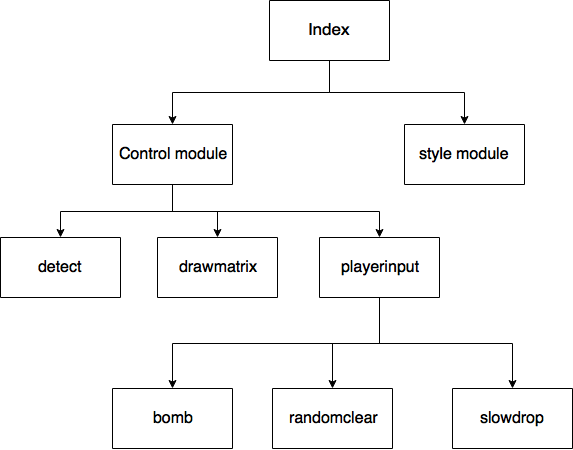
\includegraphics[width=0.7\textwidth]{UsesHierarchy.png}
\caption{Use hierarchy among modules}
\label{FigUH}
\end{figure}

%\section*{References}

\bibliographystyle {plainnat}
\bibliography {MG}

\end{document}